\documentclass[11pt]{book}
\usepackage{hyperref}
\usepackage{amsfonts}
\usepackage{amssymb}
\usepackage{amsmath}
\usepackage[utf8]{inputenc}
\usepackage[T1]{fontenc}
\usepackage{float}
\usepackage{fixltx2e}
\usepackage[italian]{babel}
\usepackage{graphicx}

\newenvironment{sistema}%
{\left\lbrace\begin{array}{@{}l@{}}}%
{\end{array}\right.}


\title{Appunti di Ricerca Operativa}
\author{Fabio Viola}
\date{}

\hyphenation{mi-ni-miz-za-re}

\setcounter{chapter}{2}

\begin{document}

\chapter{Programmazione Lineare}

\scriptsize
{\bf Slide}:
\href{http://www.or.deis.unibo.it/staff_pages/martello/Chapter3.zip}{Linear
Programming}
\normalsize
\vspace{20pt}

%% TODO Slide 1-7

\section{Problemi in due dimensioni}

$\blacktriangleright${\bf Esempio:} consideriamo il seguente problema:

\begin{center}
$min\phantom{a}z = 2x_1 - x_2 $ \\
$
  \begin{sistema}
    2x_1 + 3x_2 \leq 12 \\
    x_1, x_2 \geq 0
  \end{sistema}
$
\end{center}

Ponendo vari valori a $z$ nell'equazione $2x_1 - x_2 = z$ troviamo
varie rette parallele. In particolare un problema di questo tipo, in
due dimensioni pu\`o anche essere risolto per via grafica. La
soluzione si trova muovendosi nella direzione opposta al
gradiente. Nel nostro caso, come si vede in figura \ref{gradiente}, il
problema ha soluzione ottima in $z = -4$.

\begin{figure}
  \centering
  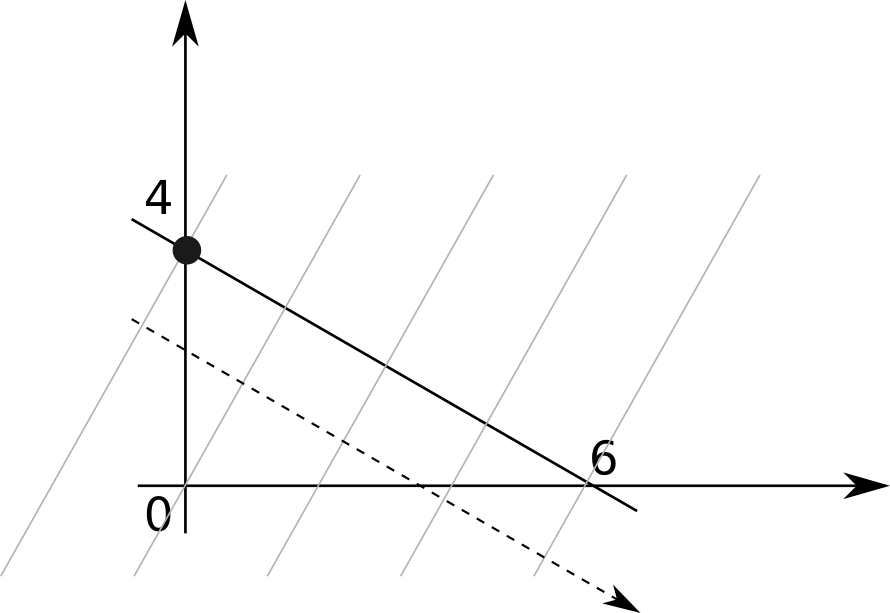
\includegraphics[width=0.65\textwidth]{images/gradiente.png}
  \caption{Risoluzione grafica}
  \label{gradiente}
\end{figure}

$\blacktriangleleft$
\newline\vspace{11pt}


\section{Forme dei problemi}

I problemi di programmazione lineare possono essere espressi in varie
forme, che elenchiamo subito:

\begin{itemize}

\item {\bf Forma generale}: 

  \begin{center}
    \begin{tabular}{l}
      $min\phantom{a}c'x$ \\
      $\phantom{aaa}a_i'x = b_i \phantom{aa} i \in M$ \\
      $\phantom{aaa}a_i'x \geq b_i \phantom{aa} i \in \bar{M}$ \\
      $\phantom{aaa}x \geq 0\phantom{aa} j \in N$\\      
      $\phantom{aaa}x \gtreqless 0\phantom{aa} j \in \bar{N}$\\      
    \end{tabular}
  \end{center}

  La forma generale ci dice che un certo numero di vincoli sono
  espressi da equazioni (quelli in cui $i \in M$), altri da
  disequazioni (dove $i \in \bar{M}$). Inoltre avremo sia variabili
  vincolate ad essere maggiori o uguali a 0 (anche minore/uguale va
  bene e ci riferiamo alle variabili $x_j$ con $j \in N$) sia
  {\bf variabili libere} ($x_j$ con $j \in \bar{N}$).

\item {\bf Forma standard}:

  \begin{center}
    \begin{tabular}{l}
      $min\phantom{a}c'x$ \\
      $\phantom{aaa}Ax = b$ \\
      $\phantom{aaa}x \geq 0$ \\      
    \end{tabular}
  \end{center}

  Nella forma standard, ma come vedremo anche nella forma canonica, le
  variabili devono obbligatoriamente assumere valori maggiori o uguali
  a 0. I vincoli che coinvolgono la matrice {\em A} devono essere
  espressi come equazioni.

\item {\bf Forma canonica}:

  \begin{center}
    \begin{tabular}{l}
      $min\phantom{a}c'x$ \\
      $\phantom{aaa}Ax \geq b$ \\
      $\phantom{aaa}x \geq 0$ \\      
    \end{tabular}
  \end{center}

  Nella forma canonica, le variabili devono obbligatoriamente assumere
  valori maggiori o uguali a 0. I vincoli che coinvolgono la matrice
  {\em A} devono essere espressi come disequazioni.
  
\end{itemize}

Le tre forme appena evidenziate sono {\bf equivalenti}, pertanto \`e
possibile passare da una all'altra e adesso vediamo come:

\begin{itemize}
  
\item {\bf dalla forma generale alla forma canonica}: \`e necessario
  trasformare le equazioni in disequazioni e lo si pu\`o fare tramite
  la sequente regola:
  \begin{center}
  $\sum\limits_{j=1}^{n}a_{ij}x_j = b_i \rightarrow 
  \begin{sistema} 
    \sum\limits_{j=1}^n a_{ij}x_j \geq b_i\\
    \sum\limits_{j=1}^n (-a_{ij})x_j \geq -b_i\\
  \end{sistema}
  $
  \end{center}
  Inoltre \`e necessario eliminare le variabili libere $x_j$ e lo si
  fa tramite l'introduzione di due variabili $x_j^+$ e $x_j^-$, come
  vediamo:
  \begin{center}
  $x_j \gtreqless 0 \rightarrow 
  \begin{sistema}
    x_j = x_j^+ - x_j^- \\
    x_j^+ \geq 0,\phantom{a}x_j^-\geq 0
  \end{sistema}
  $
  \end{center}

\item {\bf dalla forma generale alla forma standard}: \`e necessario,
  come nel caso precedente, rimuovere le variabili libere. Inoltre
  bisogna trasformare le disequazioni in equazioni. Ci\`o lo si
  realizza con l'introduzione di una {\bf slack variable} o di una
  {\bf surplus variable} $s_i$ a seconda che il segno della disequazione sia
  $\leq$ o $\geq$:

  \begin{center}
  $\sum\limits_{j=1}^n a_{ij}x_j \geq b_i \rightarrow
  \begin{sistema}
    \sum\limits_{j=1}^n a_{ij}x_j - s_i = b_i \\
    s_i \geq 0
  \end{sistema}
  $
  \end{center}

  oppure:

  \begin{center}
  $\sum\limits_{j=1}^n a_{ij}x_j \leq b_i \rightarrow
  \begin{sistema}
    \sum\limits_{j=1}^n a_{ij}x_j + s_i = b_i \\
    s_i \geq 0
  \end{sistema}
  $
  \end{center}

\end{itemize}

Vediamo con un esempio come le tre forme siano equivalenti:

\begin{center}
  
  \begin{tabular}{|l|l|l|}
    \hline
    {\bf forma generale}: & {\bf forma standard}: & {\bf forma canonica}:\\
    $min\phantom{a}x_1 + x_3$ &    $min\phantom{a}x_1 + x_3$ &    $min\phantom{a}x_1 + x_3$ \\
    $\phantom{aaaa}x_2 - 2x_3 = 4$ &    $\phantom{aaaa}x_2 - 2x_3 = 4$ &    $\phantom{aaaa}x_2 - 2x_3 \geq 4$ \\
    $\phantom{aaaa}x_1 + x_2 \geq 3$ &    $\phantom{aaaa}x_1 + x_2 - x_4 = 3$ &    $\phantom{aaaa}-x_2 + 2x_3 \geq -4$ \\
    $\phantom{aaaa}x_1, x_2, x_3 \geq 0$ &    $\phantom{aaaa}x_1, x_2,
    x_3, x_4 \geq 0$ &    $\phantom{aaaa}x_1 + x_2 \geq 3$ \\
    & &     $\phantom{aaaa}x_1, x_2, x_3 \geq 0$ \\
    \hline
  \end{tabular}

\end{center}



\section{Basi e soluzioni di base}

Nella precedente sezione abbiamo introdotto il concetto di forma
standard. Ci\`o \`e importantissimo perch\'e l'{\bf algoritmo del
  simplesso} risolve problemi in {\bf forma standard} con {\bf
  $m<n$}. Questo tuttavia non costituisce una perdita di generalit\`a
perch\'e come abbiamo visto le tre forme sono equivalenti, quindi
sar\`a sufficiente riportarci in una di queste, mentre per quanto
riguarda $m \geq n$ questo \`e un caso di scarso interesse. Non siamo
interessati n\`e a $m \geq n$ in quanto non vi sarebbero soluzioni,
n\`e a $m = n$ in quanto esisterebbe un'unica soluzione. Al contrario,
con $m < n$ esistono infinite soluzioni all'equazione $Ax=b$ ed il
sistema avrebbe $n-m$ gradi di libert\`a, intendendo con ci\`o che i
valori di $n-m$ variabili possono essere scelti
arbitrariamente. L'algoritmo del simplesso ci assicura di trovare la
soluzione ottima nell'insieme delle soluzioni ammissibili.

Per usare l'algoritmo del simplesso faremo {\bf tre assunzioni} di cui
dovremo sempre tener conto:

\begin{enumerate}
  
\item {\em A} contiene {\em m} colonne $A_j$ linearmente indipendenti,
  cio\`e il rango di {\em A} \`e esattamente {\em m}. L'algoritmo
  dev'essere in grado di rilevare violazioni alle assunzioni.

\item $F \neq 0$

\item $F$ \`e limitata nella direzione opposta (trattandosi di un
  problema di minimizzazione) al gradiente, cio\`e il valore della
  soluzione non tende a $-\infty$.

\end{enumerate}

Introduciamo il concetto di {\bf soluzioni di base}: sulla base della
prima assunzione, la matrice {\em A} contiene {\em m} colonne
linearmente indipendenti $A_j$. Definiamo {\bf base} una raccolta di
colonne linearmente indipendenti:

\begin{center}
$\mathcal{B} = \{ A_{\beta (1)}, \dots, A_{\beta (m)}\}$
\end{center}

Con $\beta(j), j=1,\dots,m$ indichiamo gli indici delle colonne che
compongono la base. La base corrisponder\`a ad una matrice di ordine
{\em m} che chiamiamo {\em B}. 

Possiamo ora definire la {\bf soluzione di base}: prendiamo in
considerazione la matrice di ordine {\em m} {\em B}. Sfruttiamo gli
$n-m$ gradi di libert\`a del sistema $Ax=b$ fissando a 0 le variabili
$x_j$ corrispondenti a {\bf variabili fuori base} (dunque $x_j = 0$
per $A_j \not\in \mathcal{B}$). Risolvendo $Bx_\beta = b$ (con
$x_\beta$ indichiamo le {\bf variabili in base} del vettore {\em x})
otteniamo un'unica soluzione $x_0$ che soddisfa $Ax = b$. Le
componenti di $x_0$ si possono calcolare con:

\begin{center}
$x_0 = B^{-1}b$
\end{center}

$x_0$ \`e la {\bf soluzione di base}. Tuttavia non \`e detto che
soddisfi il vincolo $x \geq 0$. Se lo soddisfa allora \`e detta {\bf
  soluzione di base ammissibile} o {\bf BFS} ({\em Basic Feasible
  Solution}).
\newline

\begin{figure}[h!]
  \centering
  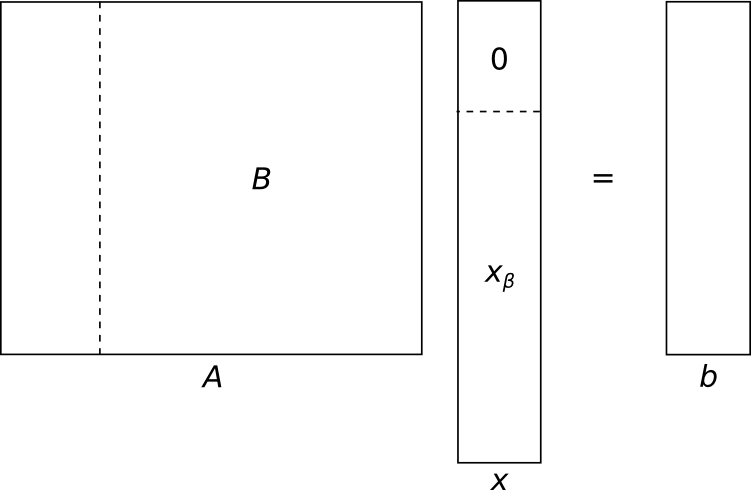
\includegraphics[width=0.5\textwidth]{images/sba.png}
\end{figure}

\vspace{11pt}
$\blacktriangleright$ {\bf Esempio:}

\begin{center}
$\begin{sistema}
x_1 + x_2 + x_3 + x_4 = 4 \\
x_1 + x_5 = 2 \\
x_3 + x_6 = 3 \\
3x_2 + x_3 + x_7 = 6 \\
x_1, x_2, x_3, x_4, x_5, x_6, x_7 \geq 0
\end{sistema}$
\end{center}

Individuiamo una base in $\mathcal{B} = \{ A_4, A_5, A_6, A_7\}$. La
corrispondente matrice $B$ \`e la {\em matrice identit\`a}. Risolvendo
$Bx = b$ otteniamo subito la soluzione di base $x =
(0,0,0,4,2,3,6)$. Questa \`e una {\bf soluzione di base
  ammissibile}. Cambiando base e scegliendo $\mathcal{B} = \{ A_2,
A_5, A_6, A_7 \}$ otteniamo:

\begin{center}$
B = \begin{bmatrix}
1 & & & \\
& 1 & & \\
& & 1 & \\
3 & & & 1 \\
\end{bmatrix}\Rightarrow
B^{-1} = 
\begin{bmatrix}
1 & & & \\
& 1 & & \\
& & 1 & \\
-3 & & & 1 \\  
\end{bmatrix}$
\end{center}

da cui ricaviamo che la soluzione base \`e $x = (0,4,0,0,2,3,-6)$ che
come vediamo {\bf non} \`e una {\em SBA}.

$\blacktriangleleft$
\newline\vspace{11pt}

\section{Politopi convessi}

Introduciamo ora un'altra definizione, quella di {\bf politopo
  convesso}. 

Dato uno spazio $\mathbb{R}^d$, un vettore di {\em d} elementi $h \neq 0$ ed uno scalare
{\em g}, un {\bf iperpiano} \`e definito da: 

\begin{center}
$\{x \in \mathbb{R}^d : h'x = g\}$
\end{center}

Un iperpiano divide lo spazio in due {\bf semispazi} definiti da $\{x
\in \mathbb{R}^d : h'x \geq g\}$ e $\{x \in \mathbb{R}^d : h'x \leq
g\}$.

%% TODO esempio 3.5

In $\mathbb{R}^2$ \`e un segmento, in $\mathbb{R}^3$ \`e un
piano e via dicendo. 

Ogni {\bf semispazio} \`e un {\bf insieme convesso} e l'intersezione
di iperspazi \`e anch'essa convessa. Un'intersezione di un numero
finito di semispazi, se limitata e non vuota, si dice {\bf politopo
  convesso}. La dimensione di un politopo \`e la minima dimensione di
uno spazio che lo pu\`o contenere (ad esempio un politopo
rappresentato da un piano non pu\`o essere rappresentato con meno di
due dimensioni, dunque la dimensione del politopo \`e 2; nel caso di
una retta, la dimensione del politopo \`e 1). Da questa osservazione
segue che la dimensione del politopo pu\`o essere inferiore allo
spazio in cui \`e rappresentato (ancora una volta pensiamo ad un piano
come politopo e immaginiamolo rappresentato in uno spazio a tre
dimensioni).
\newline\vspace{11pt}

{\bf Propriet\`a}: i vincoli di un programma di programmazione lineare definiscono un
politopo, pertanto una {\bf regione ammissibile} \`e un politopo. 
\newline\vspace{11pt}

$\square$ {\bf Dimostrazione:} \`e sufficiente ricordare che ogni
problema di programmazione lineare pu\`o essere sempre posto in forma
canonica e dunque avere una regione ammissibile definita
dall'intersezione di un insieme finito di semispazi
$\blacksquare$
\newline\vspace{11pt}

%% definizione 3.5 

{\bf Propriet\`a}: sia {\em P} un politopo. Sia {\em H} un generico
iperpiano (non ne\-ces\-sa\-ria\-men\-te associato a {\em P}) e sia
{\em HS} uno dei due semispazi definiti da {\em H}. L'insieme dei
punti $f = P \cap HS$ viene detto {\bf faccia del politopo} se:

\begin{center}
$f \not = \emptyset$ \underline{and} $f \subseteq H$
\end{center}
\vspace{11pt}

Tale relazione \`e soddisfatta soltanto se {\em H} tocca il politopo
su un suo confine.

Pi\`u informalmente diciamo che una {\bf faccia} \`e un politopo di
dimensione inferiore a {\em P} che forma un {\em bordo} di {\em P}
stesso.

Considerando un politopo di dimensione {\em d}, diciamo:

\begin{itemize}
\item {\bf faccetta}: una faccia di dimensione {\em d-1};
\item {\bf spigolo}: una faccia di dimensione 1;
\item {\bf vertice}: una faccia di dimensione 0.
\end{itemize}

%% TODO esempio 3.6

Per introdurre ulteriori propriet\`a dei {\bf politopi convessi}, \`e
necessario enunciare una {\bf generalizzazione del concetto di combinazione
convessa}: la combinazione convessa di {\em p} punti
$x^{(1)},\dots,x^{(p)} \in \mathbb{R}^n$ \`e il punto {\em z} definito
da:

\begin{center}
$z = \sum\limits_{i=1}^p \alpha_i x^{(i)}$
\end{center}

con $\sum\limits_{i=1}^p \alpha_i = 1$ e $\alpha_i \geq 0 \forall i$.

Un esempio \`e presentato in figura \ref{comb3}. Come si nota, se
prendiamo $\alpha=({1 \over 2}, 0, {1 \over 2})$, si ottiene il punto
$z={1 \over 2} (0,2) + 0 (0,0) + {1 \over 2} (4,0)=(2,1)$, mentre se
prendiamo il punto $\alpha=({1 \over 2}, {1 \over 4}, {1 \over 4})$,
si ottiene il punto $z={1 \over 2} (0,2) + {1 \over 4} (0,0) + {1
  \over 4} (4,0)=(1,1)$. In entrambi i casi i punti stanno all'interno
della figura definita dai tre punti.\newline

\begin{figure}[h!]
  \centering
  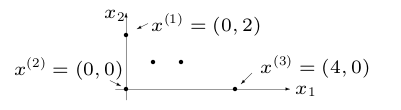
\includegraphics[width=0.6\textwidth]{images/comb3.png}
  \label{comb3}
\end{figure}

\vspace{11pt}
{\bf Teorema:} ogni punto di un politopo \`e combinazione convessa dei
vertici. Ogni combinazione convessa dei vertici \`e un punto del
politopo.
\newline\vspace{11pt}
 
{\bf Teorema:} un vertice non \`e combinazione convessa stretta
(cio\`e non \`e combinazione convessa con $0 < \lambda<1$) di due
punti distinti del politopo.
\newline

\vspace{11pt} $\square$ {\bf Dimostrazione:} dimostriamo unicamente la
sufficienza e lo faremo ragionando per assurdo. Sia {\em P} un
politopo, $v \in P$ un suo vertice e supponiamo che esistano altri due
punti $y, w \in P$ tali che:

\begin{center}
$v = \lambda y + (1 - \lambda)w$.
\end{center}

Dal momento che {\em v} \`e un vertice allora deve esistere un
semispazio $HS = \{ x : h'x \leq g\}$ tale che $HS \cup P = \{ v \}$
(se prendessimo l'altro semispazio, quello con $\geq$, l'intersezione
sarebbe tutto il politopo e non solo il vertice). Considerando ci\`o
{\em y} e {\em w} non appartengono al semispazio {\em HS}, per cui si
deve avere $h'y > g$ e $h'w > g$. Dalla tesi avremmo, moltiplicando a
destra e sinistra per {\em h'} che:

\begin{center}
$h'v = h'(\lambda y + (1-\lambda)w) = \lambda h'y + (1-\lambda)h'w >
  g$
\end{center}
da cui consegue che $v \not\in HS$, assurdo.
$\blacksquare$
\newline\vspace{11pt}

%%%%%%%%%%%%%%%%%%%%%%%%%%%%%%%%%%%%%%%%%%%%%%%%%%%%%%%%%%%%%%%%%%%%%
%%
%% RELAZIONI FRA POLITOPI E SOLUZIONI BASE
%%
%%%%%%%%%%%%%%%%%%%%%%%%%%%%%%%%%%%%%%%%%%%%%%%%%%%%%%%%%%%%%%%%%%%%%


\section{Relazioni fra politopi e soluzioni base}

Possiamo ora stabilire la relazione fondamentale tra soluzioni base e
politopi.

{\bf Propriet\`a:} l'insieme dei vincoli di un problema di programmazione lineare
definisce un politopo.

\par\bigskip 
$\square$ {\bf Dimostrazione}: \`e sufficiente osservare che la forma canonica

$$\hat F = \left\{x \in \mathbb{R}^q : \hat A x \geq b, x \geq 0
\right\}$$

con $\hat A$ matrice $ m \times q$, \`e un'intersezione di semispazi
non vuota (per l'assunzione 2) e limitata (per l'assunzione 3). $\blacksquare$
\newline

\vspace{11pt}
Si noti inoltre che $\hat F \subseteq \mathbb{R}^q$ ha dimensione $d
\leq q$. Aggiungendo {\em m} variabili surplus, si ottiene la forma
standard:

$$Ax=b \qquad con \phantom{a} A=(\hat A \mathcal j - I) \phantom{a} matrice \phantom{a} m
\times n$$ 

con $n=q+m$. Consegue dunque che, per un problema in forma standard,
la dimensione del politopo \`e $d \leq n-m$.

Passiamo ora alla relazione fondamentale tra vertici e soluzioni base.

\par\bigskip {\bf Teorema:} dato il politopo {\em P} definito dai
vincoli di un problema di programmazione lineare, condizione {\em
  necessaria e sufficiente} perch\'e un punto sia un vertice \`e che
il corrispondente vettore {\em x} sia una SBA (soluzione base
ammissibile).

\par\bigskip {\bf Dimostrazione della sufficienza:} sia
$x_{\beta}=(x_{\beta(1)},...,x_{\beta(m)})$ una SBA avente per base
l'insieme di colonne $\mathcal B = \left\{
A_{\beta(1)},...,A_{\beta(m)}\right\}$. Poich\'e {\em x} soddisfa
$Ax=b$, vale, come sappiamo gi\`a, la relazione:

$$\sum_{A_j \in \mathcal B} x_jA_j =b$$

Dimostriamo ora che {\em x} \`e un vertice, mostrando che non \`e una
combinazione convessa stretta di altri due punti distinti $ y, w
  \in P$ (come ci dice la propriet\`a dimostrata prima). Supponiamo per
assurdo che lo sia, cio\`e che esista un $\lambda$ tale che
$0 < \lambda <1$ per cui 

$$x = \lambda y + (1-\lambda)w$$

Poich\'e $x \geq 0$ deve aversi $y_j, w_j \geq 0 \phantom{i} \forall j
$. Inoltre poich\'e $x_j=0 phantom{i} \forall j \notin \mathcal B$,
deve essere anche $y_j = w_j = 0 \phantom{i} \forall j \notin \mathcal
B$.

Conseguono le due relazioni:

$$\sum_{A_j \in \mathcal B}(y_jA_j)=b \qquad e \qquad \sum_{A_j \in \mathcal B}(w_jA_j)=b$$

da cui

$$\sum_{A_j \in \mathcal B}(x_j-y_j)A_j=0 \qquad e \qquad \sum_{A_j \in \mathcal B}(x_j-w_j)A_j=0$$

Essendo le colonne $A_{\beta(1)},...,A_{\beta(m)}$ linearmente
indipendenti, qualunque loro combinazione lineare pu\`o produrre il
vettore nullo solo se tutti i coefficienti sono nulli, ossia se vale

$$x_j-y_j=x_j-w_j=0 \phantom{i} \forall j \in \mathcal B$$

da cui $x\equiv y \equiv w$, il che contraddice l'ipotesi.
\newline

{\bf Dimostrazione della necessit\`a:} dato un vertice del politopo,
sia $x \in F = \{ x \in \mathbb{R}^n : Ax = b, x \geq 0 \}$ il
corrispondente vettore, e definiamo l'insieme delle colonne di {\em A}
cui corrisponde un $x_j$ strettamente positivo: $\mathcal{C} = \{ A_j
: x_j > 0 \}$.

Dimostriamo che le colonne $A_j \in \mathcal{C}$ sono linearmente
indipendenti. Se non lo fossero, dovrebbero esistere $|\mathcal{C}|$
(numero di colonne di $\mathcal{C}$) coefficienti $d_j$ non tutti
nulli tali che:

\begin{center}
$\sum\limits_{A_j \in \mathcal{C}} d_j A_j = 0 $
\end{center}

Poich\'e $x \in F$, deve aversi $x_j \geq 0 \forall j$ e

\begin{center}
$\sum\limits_{A_j \in \mathcal{C}} x_j A_j = b$
\end{center}

Moltiplicando per uno scalare $\vartheta$ la prima sommatoria e
sommando o sottraendo il risultato dalla seconda, si ottengono:

\begin{center}
$\sum\limits_{A_j \in \mathcal{C}} (x_j + \vartheta d_j)A_j = b $  e $\sum\limits_{A_j \in \mathcal{C}} (x_j - \vartheta d_j)A_j = b $
\end{center}

Essendo $x_j > 0 \forall A_j \in \mathcal{C}$, esiste un $\vartheta$
sufficientemente piccolo per cui $x_j + \vartheta d_j \geq 0 \forall
A_j \in \mathcal{B}$ e $x_j - \vartheta d_j \geq 0 \forall A_j \in
\mathcal{B}$.

Indichiamo con $x^{(1)}$ e $x^{(2)}$ i due punti di $F$ aventi per
coordinate:

\begin{center}
$\begin{sistema}
x^{(1)}_j = x_j + \vartheta d_j,\phantom{a}x_j^{(2)} = x_j - \vartheta
d_j\phantom{aa}se\phantom{a}A_j \in \mathcal{C};

x^{(1)}_j = x_j^{(2)} = 0{aa}se\phantom{a}A_j \not \in \mathcal{C};
\end{sistema}$
\end{center}

Si ha $x = \frac{1}{2}x^{(1)}+\frac{1}{2}x^{(2)}$, cio\`e $x$ \`e
combinazione convessa stretta di due punti del politopo e quindi non
\`e un vertice, ma ci\`o \`e assurdo. Dunque le colonne $A_j \in
\mathcal{C}$ sono linearmente indipendenti e deve aversi
$|\mathcal{C}| \leq m$. Poich\'e {\em A} ha rango {\em m}, qualora si
abbia $|\mathcal{C}| < m$, possiamo aggiungere altre $m-|\mathcal{C}|$
colonne qualunque ottenendo un insieme $\mathcal{C}'$ di colonne
linearmente indipendenti con $|\mathcal{C}'|=m$ cui corrisponde lo
stesso $x$. Quindi $x$ \`e il vettore soluzione corrispondente
all'insieme $\mathcal{C}'$ di colonne linearmente indipendenti, cio\`e
ad una {\em SBA}. $\blacksquare$
\newline
\vspace{11pt}

$\blacktriangleright${\bf Esempio:} 
\begin{center}
$\begin{sistema}
2x_1 + 3x_2 + x_3 = 6 \\
x_1, x_2, x_3 \geq 0  
\end{sistema}$
\end{center}

A questo problema (in cui $n=3$ ed $m=1$) corrisponde un politopo in
$\mathbb{R}^3$. In questo problema vi sono solo tre basi possibili:
$\mathcal{B} = A_1$ in cui $x_0 = (3, 0, 0)$, $\mathcal{B} = A_2$ in
cui $x_0 = (0, 2, 0)$ e $\mathcal{B} = A_3$ in cui $x_0 = (0, 0, 6)$.
Alle tre soluzioni corrispondono i tre vertici del triangolo che
vediamo a sinistra nella figura \ref{triangolo}.

\begin{figure}[h!]
  \centering
  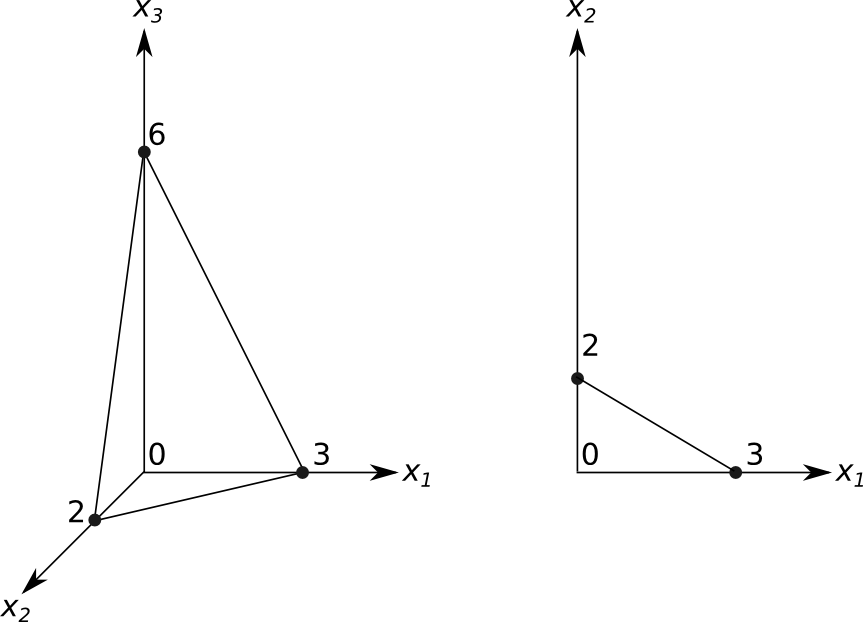
\includegraphics[width=0.6\textwidth]{images/triangolo.png}
  \label{triangolo}
\end{figure}

Prendiamo ora il seguente sistema in forma canonica:

\begin{center}
$\begin{sistema}
-2x_1 - 3x_2 \geq -6 \\
x_1, x_2 \geq 0  
\end{sistema}$
\end{center}

a cui corrisponde il politopo in figura \ref{triangolo} a destra. A
questo sistema corrisponde la forma standard seguente:

\begin{center}
$\begin{sistema}
-2x_1 - 3x_2 - s = -6 \\
x_1, x_2, s \geq 0  
\end{sistema}$
\end{center}

A livello di curiosit\`a potremmo osservare che i politopi presenti in
figura \ref{triangolo} sono identici, sono soltanto rappresentati in
spazi diversi. Il primo \`e ottenuto dal secondo trascinando il
vertice di coordinate $(0,0)$ lungo un asse perpendicolare al piano
$x_1,x_2$. In generale la forma canonica permette di vedere i politopi
in una dimensione inferiore. $\blacktriangleleft$
\newline\vspace{11pt}

\par\bigskip
{\bf Teorema:} dato un qualunque problema {\em LP}, esiste sempre un
vertice ottimo, cio\`e esiste sempre una {\em SBA} ottima.

\par\bigskip
$\square$ {\bf Dimostrazione:} sia {\em C} il vettore costo che
definisce la funzione obiettivo $min c'x$. Siano
$x^{(1)},\dots,x^{(p)}$ i vertici del politopo {\em P} determinato
dalla regione ammissibile. Sia $x^{(0)}$ il punto corrispondnte alla
soluzione ottima. Dato che $x^{(0)} \in P$ \`e possibile esprimerlo
come combinazione convessa dei vertici:

\begin{center}
$x^{(0)} = \sum\limits_{i=1}^p \alpha_i x^{(i)}$ (con
  $\sum\limits_{i=1}^p \alpha_i \geq 0, \forall i$)
\end{center}

Sia $x^{(j)}$ il vertice di costo minimo, cio\`e tale che $c'x^{(j)} =
min_{1 \leq i \leq p} \{ c'x^{(i)} \}$. Varr\`a allora:

\begin{center}
$c'x^{(0)} = c'\sum\limits_{i=1}^p \alpha_i x^{(i)} =
  \sum\limits_{i=1}^p \alpha_i c' x^{(i)} \geq c'x^{(j)}
  \sum\limits_{i=1}^p \alpha_i = c'x^{(j)}$.
\end{center}

Poich\'e non pu\`o essere $c'x^{(j)} > c'x^{(0)}$, deve aversi
$c'x^{(j)} = c'x^{(0)}$ $\blacksquare$
\newline
\vspace{11pt}

\par\bigskip {\bf Teorema:} ogni combinazione convessa di vertici
ottimi \`e ottima. (Cio\`e muovendosi lungo il segmento che unisce due
vertici ottimi si troveranno altri punti ottimi).

\par\bigskip
$\square$ {\bf Dimostrazione:} siano $x^{(1)},\dots,x^{(q)}$ vertici
ottimi e consideriamo un punto {\em x} prodotto da una loro
combinazione convessa:

\begin{center}
$x = \sum\limits_{i=1}^q \alpha_i x^{(i)}$ (con $\sum\limits_{i=1}^q
  \alpha_i = 1, \alpha_i \geq 0 \forall i$).
\end{center}

Il costo di tale punto sar\`a:

\begin{center}
$c'x = \sum\limits_{i=1}^q \alpha_i c' x^{(i)} = c' x^{(1)}
  \sum\limits_{i=1}^q \alpha_i = c'x^{(1)}$.
\end{center}
Fine dimostrazione. $\blacksquare$
\newline
\vspace{11pt}

Da questo capitolo abbiamo compreso che un problema di programmazione
lineare pu\`o essere risolto in un numero finito di passi, ad esempio
considerando tutti i vertici di un politopo e scegliendo la {\em SBA}
di costo minimo. Tuttavia esaminare tutti i possibili vertici
richiederebbe un tempo di esecuzione molto elevato, per questo noi
utilizzeremo il metodo del simplesso che invece procede in maniera
intelligente alla ricerca della soluzione ottima.

%%%%%%%%%%%%%%%%%%%%%%%%%%%%%%%%%%%%%%%%%%%%%%%%%%%%%%%%%%%%%%%%%%%%%
%%
%% BASI DEGENERI
%%
%%%%%%%%%%%%%%%%%%%%%%%%%%%%%%%%%%%%%%%%%%%%%%%%%%%%%%%%%%%%%%%%%%%%%

\section{Basi degeneri}

Una base $\mathcal{B}$ determina univocamente una soluzione base, per
cui se due {\em SBA} sono diverse, sono sicuramente prodotte da basi
diverse. Non \`e vero invece il contrario, ovvero che, date due basi
distinte, esse producano sempre due {\em SBA} distinte.

{\em Normalmente} una {\em SBA} ha soltanto {\em n-m} zeri, quelli
dati dall'aver posto a 0 le variabili fuori base. Le basi degeneri
hanno invece anche alcune variabili in base pari a 0. Pertanto
definiamo {\bf base degenere}, una base che contenga pi\`u di {\em
  n-m} variabili con valore 0.
\newline

\vspace{11pt}
{\bf Propriet\`a}: se due basi distinte $\mathcal{B}$ e
$\bar{\mathcal{B}}$ producono la stessa {\em SBA x}, allora {\em x}
\`e degenere.
\newline

\vspace{11pt} $\square$ {\bf Dimostrazione:} la soluzione {\em x} ha
sicuramente {\em n-m} zeri in corrispondenza delle colonne che non
sono in $\mathcal{B}$. Inoltre anche per le colonne non in
$\bar{\mathcal{B}}$ avremo 0. Essendo disgiunte le due basi, questo
vuol dire che avremo pi\`u di $n-m$ zeri, dunque che {\em x} \`e
degenere.  $\blacksquare$
\newline\vspace{11pt}

\end{document}
